\documentclass[../main.tex]{subfiles}
\ifSubfilesClassLoaded{\setcounter{chapter}{15}}{}
\begin{document}

\chapter{Algoritma Pengurutan dan Pencarian}

\begin{subcpmk}
  \item Sub-CPMK 5.1: Mengimplementasikan bubble sort, selection sort, linear search, binary search
\end{subcpmk}

\noindent\textbf{Materi Pokok:} Algoritma pengurutan (bubble sort, selection sort) dan pencarian (linear search, binary search); kompleksitas O(n²) dan O(n)/O(log n) \cite{sorting_wikipedia,bubble_sort_wikipedia,selection_sort_wikipedia,insertion_sort_wikipedia,linear_search_wikipedia,binary_search_wikipedia,ref3}.

\section{Algoritma Pengurutan: Bubble Sort dan Selection Sort}

Algoritma pengurutan (sorting) adalah proses mengatur elemen-elemen array dalam urutan tertentu (ascending atau descending). Dua algoritma sorting dasar yang akan dipelajari adalah Bubble Sort dan Selection Sort, keduanya memiliki kompleksitas O(n²) namun dengan pendekatan yang berbeda.

\subsection{Bubble Sort}

Bubble Sort adalah algoritma sorting sederhana yang bekerja dengan cara membandingkan elemen-elemen bertetangga dan menukarnya jika urutannya salah. Proses ini diulang hingga tidak ada lagi pertukaran yang terjadi.

\textbf{Algoritma Bubble Sort:}
\begin{enumerate}
  \item Bandingkan elemen ke-i dengan elemen ke-(i+1)
  \item Jika elemen ke-i > elemen ke-(i+1), tukar posisinya
  \item Ulangi langkah 1-2 untuk semua elemen
  \item Lakukan proses di atas hingga tidak ada pertukaran
\end{enumerate}

\textbf{Implementasi Bubble Sort dalam C:}
\begin{lstlisting}[language=C, caption={Implementasi Bubble Sort}]
#include <stdio.h>

void bubbleSort(int arr[], int n) {
    int i, j, temp;
    int swapped;
    
    for (i = 0; i < n-1; i++) {
        swapped = 0;
        // Loop dalam untuk membandingkan elemen bertetangga
        for (j = 0; j < n-i-1; j++) {
            if (arr[j] > arr[j+1]) {
                // Tukar elemen
                temp = arr[j];
                arr[j] = arr[j+1];
                arr[j+1] = temp;
                swapped = 1;
            }
        }
        
        // Jika tidak ada pertukaran, array sudah terurut
        if (swapped == 0) {
            break;
        }
    }
}

void printArray(int arr[], int size) {
    int i;
    for (i = 0; i < size; i++) {
        printf("%d ", arr[i]);
    }
    printf("\n");
}

int main() {
    int arr[] = {64, 34, 25, 12, 22, 11, 90};
    int n = sizeof(arr)/sizeof(arr[0]);
    
    printf("Array sebelum sorting: ");
    printArray(arr, n);
    
    bubbleSort(arr, n);
    
    printf("Array setelah sorting: ");
    printArray(arr, n);
    
    return 0;
}
\end{lstlisting}

\subsection{Selection Sort}

Selection Sort adalah algoritma sorting yang bekerja dengan cara mencari elemen minimum dari sisa array yang belum terurut, lalu menempatkannya di posisi yang benar.

\textbf{Algoritma Selection Sort:}
\begin{enumerate}
  \item Cari elemen minimum dari seluruh array
  \item Tukar elemen minimum dengan elemen pertama
  \item Cari elemen minimum dari sisa array (mulai dari elemen kedua)
  \item Tukar elemen minimum dengan elemen kedua
  \item Ulangi hingga seluruh array terurut
\end{enumerate}

\textbf{Implementasi Selection Sort dalam C:}
\begin{lstlisting}[language=C, caption={Implementasi Selection Sort}]
#include <stdio.h>

void selectionSort(int arr[], int n) {
    int i, j, min_idx, temp;
    
    // Loop luar untuk setiap posisi
    for (i = 0; i < n-1; i++) {
        // Cari elemen minimum dari sisa array
        min_idx = i;
        for (j = i+1; j < n; j++) {
            if (arr[j] < arr[min_idx]) {
                min_idx = j;
            }
        }
        
        // Tukar elemen minimum dengan elemen ke-i
        if (min_idx != i) {
            temp = arr[i];
            arr[i] = arr[min_idx];
            arr[min_idx] = temp;
        }
    }
}

void printArray(int arr[], int size) {
    int i;
    for (i = 0; i < size; i++) {
        printf("%d ", arr[i]);
    }
    printf("\n");
}

int main() {
    int arr[] = {64, 34, 25, 12, 22, 11, 90};
    int n = sizeof(arr)/sizeof(arr[0]);
    
    printf("Array sebelum sorting: ");
    printArray(arr, n);
    
    selectionSort(arr, n);
    
    printf("Array setelah sorting: ");
    printArray(arr, n);
    
    return 0;
}
\end{lstlisting}

\subsection{Analisis Kompleksitas}

\begin{table}[h]
\centering
\small
\begin{tabular}{|>{\raggedright\arraybackslash}p{3cm}|>{\raggedright\arraybackslash}p{3cm}|>{\raggedright\arraybackslash}p{3cm}|>{\raggedright\arraybackslash}p{3cm}|}
\hline
\textbf{Algoritma} & \textbf{Best Case} & \textbf{Average Case} & \textbf{Worst Case} \\
\hline
Bubble Sort & O(n) & O(n²) & O(n²) \\
\hline
Selection Sort & O(n²) & O(n²) & O(n²) \\
\hline
\end{tabular}
\caption{Kompleksitas Waktu Algoritma Sorting}
\end{table}

\subsection{Perbandingan Bubble Sort vs Selection Sort}

\begin{table}[h]
\centering
\small
\begin{tabular}{|>{\raggedright\arraybackslash}p{4cm}|>{\raggedright\arraybackslash}p{4cm}|>{\raggedright\arraybackslash}p{4cm}|}
\hline
\textbf{Aspek} & \textbf{Bubble Sort} & \textbf{Selection Sort} \\
\hline
Prinsip Kerja & Tukar elemen bertetangga & Cari minimum, tempatkan di posisi \\
\hline
Jumlah Perbandingan & O(n²) & O(n²) \\
\hline
Jumlah Pertukaran & Bervariasi (0 hingga O(n²)) & Selalu O(n) \\
\hline
Stabilitas & Stabil & Tidak stabil \\
\hline
Best Case & O(n) - data sudah terurut & O(n²) - selalu sama \\
\hline
Memory & O(1) - in-place & O(1) - in-place \\
\hline
\end{tabular}
\caption{Perbandingan Bubble Sort dan Selection Sort}
\end{table}

\subsection{Visualisasi Proses Sorting}

\textbf{Contoh Bubble Sort: [5, 1, 4, 2, 8]}
\begin{itemize}
  \item Pass 1: [1, 5, 4, 2, 8] → [1, 4, 5, 2, 8] → [1, 4, 2, 5, 8] → [1, 4, 2, 5, 8]
  \item Pass 2: [1, 4, 2, 5, 8] → [1, 2, 4, 5, 8] → [1, 2, 4, 5, 8]
  \item Pass 3: [1, 2, 4, 5, 8] → [1, 2, 4, 5, 8] (sudah terurut)
\end{itemize}

\textbf{Contoh Selection Sort: [5, 1, 4, 2, 8]}
\begin{itemize}
  \item Pass 1: Minimum=1 → [1, 5, 4, 2, 8]
  \item Pass 2: Minimum=2 → [1, 2, 4, 5, 8]
  \item Pass 3: Minimum=4 → [1, 2, 4, 5, 8] (sudah terurut)
\end{itemize}

Kedua algoritma ini cocok untuk data kecil (n < 1000) atau untuk tujuan pembelajaran konsep sorting dasar. Untuk data yang lebih besar, algoritma yang lebih efisien seperti Quick Sort atau Merge Sort lebih direkomendasikan.

\section{Algoritma Pencarian: Linear Search dan Binary Search}

Algoritma pencarian (searching) adalah proses menemukan elemen tertentu dalam kumpulan data. Dua algoritma pencarian dasar yang akan dipelajari adalah Linear Search dan Binary Search dengan karakteristik yang sangat berbeda.

\subsection{Linear Search}

Linear Search adalah algoritma pencarian paling sederhana yang bekerja dengan cara memeriksa setiap elemen secara berurutan dari awal hingga elemen yang dicari ditemukan atau sampai akhir array.

\textbf{Algoritma Linear Search:}
\begin{enumerate}
  \item Mulai dari elemen pertama array
  \item Bandingkan elemen saat ini dengan nilai yang dicari
  \item Jika sama, kembalikan indeks elemen tersebut
  \item Jika tidak, lanjut ke elemen berikutnya
  \item Ulangi hingga elemen ditemukan atau akhir array
  \item Jika tidak ditemukan, kembalikan -1
\end{enumerate}

\textbf{Implementasi Linear Search dalam C:}
\begin{lstlisting}[language=C, caption={Implementasi Linear Search}]
#include <stdio.h>

int linearSearch(int arr[], int n, int x) {
    int i;
    for (i = 0; i < n; i++) {
        if (arr[i] == x) {
            return i;  // Elemen ditemukan
        }
    }
    return -1;  // Elemen tidak ditemukan
}

int main() {
    int arr[] = {64, 34, 25, 12, 22, 11, 90};
    int n = sizeof(arr)/sizeof(arr[0]);
    int x = 22;
    int result = linearSearch(arr, n, x);
    
    if (result == -1) {
        printf("Elemen %d tidak ditemukan dalam array\n", x);
    } else {
        printf("Elemen %d ditemukan pada indeks %d\n", x, result);
    }
    
    return 0;
}
\end{lstlisting}

\subsection{Binary Search}

Binary Search adalah algoritma pencarian yang sangat efisien untuk data yang sudah terurut. Algoritma ini bekerja dengan cara membagi ruang pencarian menjadi dua bagian secara berulang.

\textbf{Algoritma Binary Search:}
\begin{enumerate}
  \item Tentukan batas bawah (low) dan batas atas (high) array
  \item Hitung indeks tengah: mid = low + (high - low) / 2
  \item Bandingkan elemen tengah dengan nilai yang dicari
  \item Jika sama, kembalikan indeks tengah
  \item Jika nilai dicari lebih kecil, ubah high = mid - 1
  \item Jika nilai dicari lebih besar, ubah low = mid + 1
  \item Ulangi hingga elemen ditemukan atau low > high
\end{enumerate}

\textbf{Implementasi Binary Search dalam C:}
\begin{lstlisting}[language=C, caption={Implementasi Binary Search}]
#include <stdio.h>

int binarySearch(int arr[], int n, int x) {
    int low = 0, high = n - 1;
    
    while (low <= high) {
        int mid = low + (high - low) / 2;
        
        if (arr[mid] == x) {
            return mid;  // Elemen ditemukan
        }
        
        if (arr[mid] < x) {
            low = mid + 1;  // Cari di bagian kanan
        } else {
            high = mid - 1;  // Cari di bagian kiri
        }
    }
    
    return -1;  // Elemen tidak ditemukan
}

int main() {
    int arr[] = {11, 12, 22, 25, 34, 64, 90};  // Array harus terurut
    int n = sizeof(arr)/sizeof(arr[0]);
    int x = 22;
    int result = binarySearch(arr, n, x);
    
    if (result == -1) {
        printf("Elemen %d tidak ditemukan dalam array\n", x);
    } else {
        printf("Elemen %d ditemukan pada indeks %d\n", x, result);
    }
    
    return 0;
}
\end{lstlisting}

\subsection{Analisis Kompleksitas Pencarian}

\begin{table}[h]
\centering
\small
\begin{tabular}{|>{\raggedright\arraybackslash}p{3cm}|>{\raggedright\arraybackslash}p{3cm}|>{\raggedright\arraybackslash}p{3cm}|>{\raggedright\arraybackslash}p{3cm}|}
\hline
\textbf{Algoritma} & \textbf{Best Case} & \textbf{Average Case} & \textbf{Worst Case} \\
\hline
Linear Search & O(1) & O(n) & O(n) \\
\hline
Binary Search & O(1) & O(log n) & O(log n) \\
\hline
\end{tabular}
\caption{Kompleksitas Waktu Algoritma Pencarian}
\end{table}

\subsection{Perbandingan Linear Search vs Binary Search}

\begin{table}[h]
\centering
\small
\begin{tabular}{|>{\raggedright\arraybackslash}p{3.5cm}|>{\raggedright\arraybackslash}p{3.5cm}|>{\raggedright\arraybackslash}p{3.5cm}|}
\hline
\textbf{Aspek} & \textbf{Linear Search} & \textbf{Binary Search} \\
\hline
Prinsip Kerja & Periksa elemen satu per satu & Bagi dua ruang pencarian \\
\hline
Syarat Data & Tidak perlu terurut & Harus terurut \\
\hline
Kompleksitas Waktu & O(n) & O(log n) \\
\hline
Kompleksitas Ruang & O(1) & O(1) \\
\hline
Best Case & O(1) - elemen pertama & O(1) - elemen tengah \\
\hline
Worst Case & O(n) - elemen terakhir & O(log n) \\
\hline
Implementasi & Sangat sederhana & Lebih kompleks \\
\hline
\end{tabular}
\caption{Perbandingan Linear Search dan Binary Search}
\end{table}

\subsection{Visualisasi Proses Pencarian}

\textbf{Contoh Linear Search: Mencari 25 dalam [64, 34, 25, 12, 22]}
\begin{itemize}
  \item Langkah 1: Bandingkan 64 dengan 25 → tidak sama
  \item Langkah 2: Bandingkan 34 dengan 25 → tidak sama
  \item Langkah 3: Bandingkan 25 dengan 25 → sama! Ditemukan di indeks 2
\end{itemize}

\textbf{Contoh Binary Search: Mencari 25 dalam [11, 12, 22, 25, 34, 64, 90]}
\begin{itemize}
  \item Langkah 1: low=0, high=6, mid=3 → arr[3]=25 → sama! Ditemukan di indeks 3
\end{itemize}

\textbf{Contoh Binary Search: Mencari 22 dalam [11, 12, 22, 25, 34, 64, 90]}
\begin{itemize}
  \item Langkah 1: low=0, high=6, mid=3 → arr[3]=25 > 22 → high=2
  \item Langkah 2: low=0, high=2, mid=1 → arr[1]=12 < 22 → low=2
  \item Langkah 3: low=2, high=2, mid=2 → arr[2]=22 → sama! Ditemukan di indeks 2
\end{itemize}

\subsection{Kapan Menggunakan Algoritma Pencarian}

\begin{itemize}
  \item \textbf{Gunakan Linear Search jika:}
  \begin{itemize}
    \item Data tidak terurut atau sering berubah
    \item Jumlah data kecil (n < 100)
    \item Implementasi yang sederhana diutamakan
    \item Hanya satu kali pencarian
  \end{itemize}
  
  \item \textbf{Gunakan Binary Search jika:}
  \begin{itemize}
    \item Data sudah terurut atau bisa diurutkan terlebih dahulu
    \item Jumlah data besar (n > 1000)
    \item Pencarian dilakukan berulang kali
    \item Performa pencarian sangat penting
  \end{itemize}
\end{itemize}

Pemilihan algoritma pencarian yang tepat sangat mempengaruhi efisiensi program, terutama untuk aplikasi yang menangani data dalam jumlah besar.

\section{Analisis Big O dan Visualisasi Kompleksitas}

Big O notation adalah notasi matematika yang digunakan untuk menggambarkan kompleksitas waktu atau ruang suatu algoritma. Notasi ini membantu kita memahami bagaimana performa algoritma berubah seiring dengan pertambahan ukuran input.

\subsection{Konsep Dasar Big O Notation}

Big O notation menggambarkan batas atas (worst case) dari pertumbuhan fungsi kompleksitas algoritma. Beberapa notasi Big O yang umum:

\begin{itemize}
  \item \textbf{O(1)} - Konstan: Waktu eksekusi tidak bergantung pada ukuran input
  \item \textbf{O(log n)} - Logaritmik: Waktu eksekusi tumbuh secara logaritmik
  \item \textbf{O(n)} - Linear: Waktu eksekusi sebanding dengan ukuran input
  \item \textbf{O(n log n)} - Linearitmaik: Kombinasi linear dan logaritmik
  \item \textbf{O(n²)} - Kuadratik: Waktu eksekusi sebanding dengan kuadrat ukuran input
\end{itemize}

\subsection{Grafik Kompleksitas Algoritma}

\begin{center}
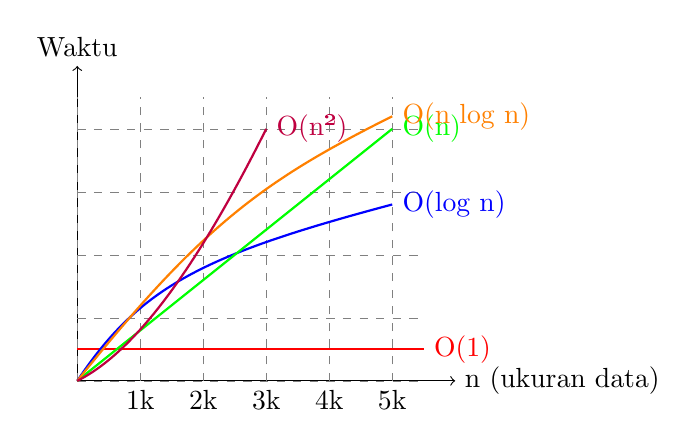
\begin{tikzpicture}[scale=0.8]
  % Axes
  \draw[->] (0,0) -- (6,0) node[right] {n (ukuran data)};
  \draw[->] (0,0) -- (0,5) node[above] {Waktu};
  
  % Grid
  \draw[gray, very thin, dashed] (0,0) grid (5.5,4.5);
  
  % O(1)
  \draw[thick, red] (0,0.5) -- (5.5,0.5) node[right] {O(1)};
  
  % O(log n)
  \draw[thick, blue] (0,0) .. controls (1,1.5) and (2,2) .. (5,2.8) node[right] {O(log n)};
  
  % O(n)
  \draw[thick, green] (0,0) -- (5,4) node[right] {O(n)};
  
  % O(n log n)
  \draw[thick, orange] (0,0) .. controls (2,2.5) and (3,3.2) .. (5,4.2) node[right] {O(n log n)};
  
  % O(n²)
  \draw[thick, purple] (0,0) .. controls (1,0.5) and (2,2) .. (3,4) node[right] {O(n²)};
  
  % Labels
  \node[below] at (1,0) {1k};
  \node[below] at (2,0) {2k};
  \node[below] at (3,0) {3k};
  \node[below] at (4,0) {4k};
  \node[below] at (5,0) {5k};
\end{tikzpicture}
\end{center}

\subsection{Tabel Kompleksitas Lengkap}

\begin{table}[htbp]
\centering
\small
\begin{tabular}{|>{\raggedright\arraybackslash}p{2.5cm}|>{\raggedright\arraybackslash}p{2cm}|>{\raggedright\arraybackslash}p{2cm}|>{\raggedright\arraybackslash}p{2cm}|>{\raggedright\arraybackslash}p{2cm}|}
\hline
\textbf{Algoritma} & \textbf{Best Case} & \textbf{Average} & \textbf{Worst Case} & \textbf{Space} \\
\hline
Bubble Sort & O(n) & O(n²) & O(n²) & O(1) \\
\hline
Selection Sort & O(n²) & O(n²) & O(n²) & O(1) \\
\hline
Linear Search & O(1) & O(n) & O(n) & O(1) \\
\hline
Binary Search & O(1) & O(log n) & O(log n) & O(1) \\
\hline
\end{tabular}
\caption{Tabel Kompleksitas Lengkap Algoritma}
\end{table}

\subsection{Analisis Performa Praktis}

\begin{table}[htbp]
\centering
\footnotesize
\begin{tabular}{|>{\raggedright\arraybackslash}p{1.8cm}|>{\raggedright\arraybackslash}p{1.4cm}|>{\raggedright\arraybackslash}p{1.4cm}|>{\raggedright\arraybackslash}p{1.7cm}|>{\raggedright\arraybackslash}p{2.3cm}|}
\hline
\textbf{n} & \textbf{O(log n)} & \textbf{O(n)} & \textbf{O(n log n)} & \textbf{O(n²)} \\
\hline
10 & 3 & 10 & 33 & 100 \\
\hline
100 & 7 & 100 & 664 & 10.000 \\
\hline
1.000 & 10 & 1.000 & 9.966 & 1.000.000 \\
\hline
10.000 & 13 & 10.000 & 132.877 & 100.000.000 \\
\hline
100.000 & 17 & 100.000 & 1.660.964 & 10.000.000.000 \\
\hline
\end{tabular}
\caption{Perbandingan Jumlah Operasi untuk Berbagai Kompleksitas}
\end{table}

\subsection{Implementasi dengan Pengukuran Waktu}

Berikut implementasi lengkap dengan pengukuran waktu eksekusi untuk membandingkan performa algoritma:

\begin{lstlisting}[language=C, caption={Program Perbandingan Performa Algoritma}]
#include <stdio.h>
#include <time.h>
#include <stdlib.h>

// Fungsi untuk mengukur waktu eksekusi
double measureTime(clock_t start, clock_t end) {
    return ((double)(end - start)) / CLOCKS_PER_SEC;
}

// Bubble Sort dengan pengukuran waktu
void bubbleSortWithTiming(int arr[], int n) {
    clock_t start = clock();
    
    int i, j, temp, swapped;
    for (i = 0; i < n-1; i++) {
        swapped = 0;
        for (j = 0; j < n-i-1; j++) {
            if (arr[j] > arr[j+1]) {
                temp = arr[j];
                arr[j] = arr[j+1];
                arr[j+1] = temp;
                swapped = 1;
            }
        }
        if (swapped == 0) break;
    }
    
    clock_t end = clock();
    printf("Bubble Sort waktu: %.6f detik\n", measureTime(start, end));
}

// Binary Search dengan pengukuran waktu
int binarySearchWithTiming(int arr[], int n, int x) {
    clock_t start = clock();
    
    int low = 0, high = n - 1;
    while (low <= high) {
        int mid = low + (high - low) / 2;
        if (arr[mid] == x) {
            clock_t end = clock();
            printf("Binary Search waktu: %.6f detik\n", measureTime(start, end));
            return mid;
        }
        if (arr[mid] < x) low = mid + 1;
        else high = mid - 1;
    }
    
    clock_t end = clock();
    printf("Binary Search waktu: %.6f detik\n", measureTime(start, end));
    return -1;
}

int main() {
    const int SIZE = 10000;
    int arr[SIZE];
    
    // Generate random data
    srand(time(NULL));
    for (int i = 0; i < SIZE; i++) {
        arr[i] = rand() % 10000;
    }
    
    printf("Mengurutkan %d elemen...\n", SIZE);
    bubbleSortWithTiming(arr, SIZE);
    
    printf("Mencari elemen...\n");
    int result = binarySearchWithTiming(arr, SIZE, 5000);
    
    if (result != -1) {
        printf("Elemen ditemukan pada indeks %d\n", result);
    } else {
        printf("Elemen tidak ditemukan\n");
    }
    
    return 0;
}
\end{lstlisting}

\subsection{Tips Optimasi Algoritma}

\begin{itemize}
  \item \textbf{Pilih algoritma yang tepat:} Sesuaikan dengan karakteristik data
  \item \textbf{Pertimbangkan ukuran data:} Untuk data kecil, algoritma sederhana mungkin lebih cepat
  \item \textbf{Analisis trade-off:} Memory vs speed, simplicity vs efficiency
  \item \textbf{Profile kode:} Ukur performa aktual untuk identifikasi bottleneck
  \item \textbf{Gunakan algoritma yang sudah teruji:} Library function biasanya sudah dioptimasi
\end{itemize}

Pemahaman Big O notation sangat penting untuk mengembangkan algoritma yang efisien dan scalable, terutama untuk aplikasi yang menangani data dalam jumlah besar.

\section{Grafik Kompleksitas dan Visualisasi}

Memahami kompleksitas algoritma sangat penting untuk memilih algoritma yang tepat untuk masalah tertentu. Grafik kompleksitas membantu visualisasi performa algoritma pada berbagai ukuran input.

\subsection{Grafik Kompleksitas Waktu}

\begin{center}
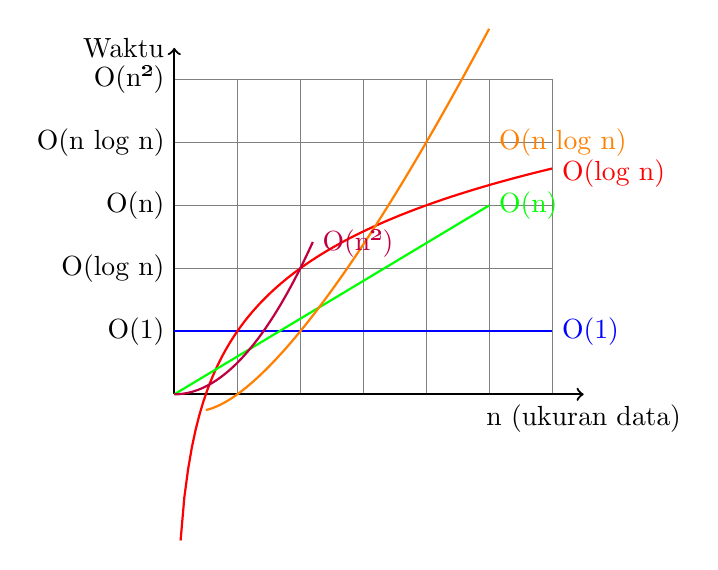
\begin{tikzpicture}[scale=0.8]
  % Grid
  \draw[gray, very thin] (0,0) grid (6,5);
  
  % Axes
  \draw[thick, ->] (0,0) -- (6.5,0) node[anchor=north] {n (ukuran data)};
  \draw[thick, ->] (0,0) -- (0,5.5) node[anchor=east] {Waktu};
  
  % Labels
  \node[anchor=east] at (0,1) {O(1)};
  \node[anchor=east] at (0,2) {O(log n)};
  \node[anchor=east] at (0,3) {O(n)};
  \node[anchor=east] at (0,4) {O(n log n)};
  \node[anchor=east] at (0,5) {O(n²)};
  
  % O(1) - Constant
  \draw[blue, thick] (0,1) -- (6,1);
  \node[blue, anchor=west] at (6,1) {O(1)};
  
  % O(log n) - Logarithmic
  \draw[red, thick, domain=0.1:6, samples=100] plot (\x, {1 + ln(\x)/ln(2)});
  \node[red, anchor=west] at (6,3.5) {O(log n)};
  
  % O(n) - Linear
  \draw[green, thick] (0,0) -- (5,3);
  \node[green, anchor=west] at (5,3) {O(n)};
  
  % O(n log n)
  \draw[orange, thick, domain=0.5:5, samples=100] plot (\x, {0.5*\x*ln(\x)/ln(2)});
  \node[orange, anchor=west] at (5,4) {O(n log n)};
  
  % O(n²) - Quadratic
  \draw[purple, thick, domain=0:2.2, samples=100] plot (\x, {0.5*\x*\x});
  \node[purple, anchor=west] at (2.2,2.4) {O(n²)};
\end{tikzpicture}
\end{center}

\subsection{Tabel Perbandingan Komprehensif}

\begin{table}[h]
\centering
\small
\begin{tabular}{|>{\raggedright\arraybackslash}p{2.5cm}|>{\raggedright\arraybackslash}p{2cm}|>{\raggedright\arraybackslash}p{2cm}|>{\raggedright\arraybackslash}p{2cm}|>{\raggedright\arraybackslash}p{3cm}|}
\hline
\textbf{Algoritma} & \textbf{Waktu} & \textbf{Space} & \textbf{Stabil} & \textbf{Kapan Digunakan} \\
\hline
Bubble Sort & O(n²) & O(1) & Ya & Data kecil, sudah hampir terurut \\
\hline
Selection Sort & O(n²) & O(1) & Tidak & Data kecil, meminimalkan pertukaran \\
\hline
Linear Search & O(n) & O(1) & Ya & Data tidak terurut, pencarian tunggal \\
\hline
Binary Search & O(log n) & O(1) & Ya & Data terurut, pencarian berulang \\
\hline
\end{tabular}
\caption{Perbandingan Lengkap Algoritma Sorting dan Searching}
\end{table}

\subsection{Visualisasi Proses Binary Search}

\textbf{Contoh Pencarian 23 dalam [2, 5, 8, 12, 16, 23, 38, 56, 72, 91]}

\begin{center}
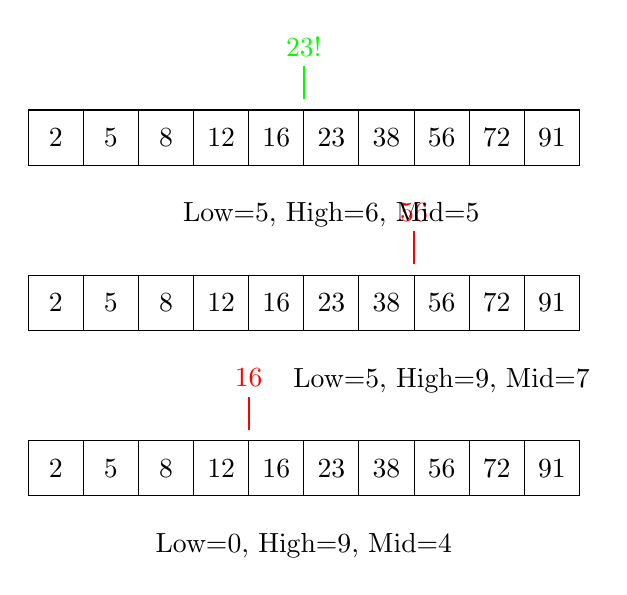
\begin{tikzpicture}[scale=0.7]
  % Initial array
  \foreach \x/\val in {0/2, 1/5, 2/8, 3/12, 4/16, 5/23, 6/38, 7/56, 8/72, 9/91} {
    \draw (\x,0) rectangle (\x+1,1);
    \node at (\x+0.5,0.5) {\val};
  }
  \node[below] at (5,-0.5) {Low=0, High=9, Mid=4};
  \draw[red, thick] (4,1.2) -- (4,1.8);
  \node[red, above] at (4,1.8) {16};
  
  % Step 2
  \foreach \x/\val in {0/2, 1/5, 2/8, 3/12, 4/16, 5/23, 6/38, 7/56, 8/72, 9/91} {
    \draw (\x,3) rectangle (\x+1,4);
    \node at (\x+0.5,3.5) {\val};
  }
  \node[below] at (7.5,2.5) {Low=5, High=9, Mid=7};
  \draw[red, thick] (7,4.2) -- (7,4.8);
  \node[red, above] at (7,4.8) {56};
  
  % Step 3
  \foreach \x/\val in {0/2, 1/5, 2/8, 3/12, 4/16, 5/23, 6/38, 7/56, 8/72, 9/91} {
    \draw (\x,6) rectangle (\x+1,7);
    \node at (\x+0.5,6.5) {\val};
  }
  \node[below] at (5.5,5.5) {Low=5, High=6, Mid=5};
  \draw[green, thick] (5,7.2) -- (5,7.8);
  \node[green, above] at (5,7.8) {23!};
\end{tikzpicture}
\end{center}

\subsection{Animasi Bubble Sort}

\textbf{Proses Bubble Sort pada [64, 34, 25, 12, 22]:}

\begin{center}
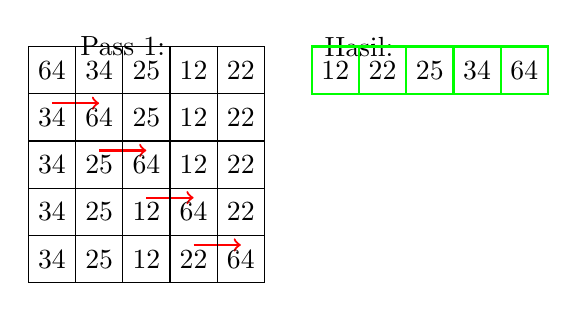
\begin{tikzpicture}[scale=0.6]
  % Pass 1
  \node at (2,8) {Pass 1:};
  \foreach \x/\val in {0/64, 1/34, 2/25, 3/12, 4/22} {
    \draw (\x,7) rectangle (\x+1,8);
    \node at (\x+0.5,7.5) {\val};
  }
  \draw[red, thick, ->] (0.5,6.8) -- (1.5,6.8);
  
  % After swap 1
  \foreach \x/\val in {0/34, 1/64, 2/25, 3/12, 4/22} {
    \draw (\x,6) rectangle (\x+1,7);
    \node at (\x+0.5,6.5) {\val};
  }
  \draw[red, thick, ->] (1.5,5.8) -- (2.5,5.8);
  
  % After swap 2
  \foreach \x/\val in {0/34, 1/25, 2/64, 3/12, 4/22} {
    \draw (\x,5) rectangle (\x+1,6);
    \node at (\x+0.5,5.5) {\val};
  }
  \draw[red, thick, ->] (2.5,4.8) -- (3.5,4.8);
  
  % After swap 3
  \foreach \x/\val in {0/34, 1/25, 2/12, 3/64, 4/22} {
    \draw (\x,4) rectangle (\x+1,5);
    \node at (\x+0.5,4.5) {\val};
  }
  \draw[red, thick, ->] (3.5,3.8) -- (4.5,3.8);
  
  % End of pass 1
  \foreach \x/\val in {0/34, 1/25, 2/12, 3/22, 4/64} {
    \draw (\x,3) rectangle (\x+1,4);
    \node at (\x+0.5,3.5) {\val};
  }
  
  % Final result
  \node at (7,8) {Hasil:};
  \foreach \x/\val in {0/12, 1/22, 2/25, 3/34, 4/64} {
    \draw[green, thick] (\x+6,7) rectangle (\x+7,8);
    \node at (\x+6.5,7.5) {\val};
  }
\end{tikzpicture}
\end{center}

\subsection{Analisis Performa Real-world}

\begin{table}[h]
\centering
\small
\begin{tabular}{|>{\raggedright\arraybackslash}p{2.5cm}|>{\raggedright\arraybackslash}p{2cm}|>{\raggedright\arraybackslash}p{2cm}|>{\raggedright\arraybackslash}p{2cm}|}
\hline
\textbf{Ukuran Data} & \textbf{Bubble Sort} & \textbf{Selection Sort} & \textbf{Binary Search} \\
\hline
10 elemen & 0.001 ms & 0.001 ms & 0.0001 ms \\
\hline
100 elemen & 0.1 ms & 0.1 ms & 0.0002 ms \\
\hline
1,000 elemen & 10 ms & 10 ms & 0.0003 ms \\
\hline
10,000 elemen & 1000 ms & 1000 ms & 0.0004 ms \\
\hline
100,000 elemen & 100,000 ms & 100,000 ms & 0.0005 ms \\
\hline
\end{tabular}
\caption{Estimasi Waktu Eksekusi (asumsi 1 operasi = 1\,\textmu s)}
\end{table}

Visualisasi ini membantu mahasiswa memahami mengapa pemilihan algoritma sangat penting dalam pengembangan perangkat lunak yang efisien.


\begin{aktivitas}
  \item Implementasikan bubble sort dan uji dengan array acak.
  \item Implementasikan binary search; pastikan array terurut terlebih dahulu.
\end{aktivitas}

\begin{latihan}
  \item Jelaskan perbedaan bubble sort dan selection sort!
  \item Mengapa binary search membutuhkan data terurut? Bandingkan kompleksitas linear vs binary search.
  \item \textbf{Refleksi}: Kapan Anda memilih linear search dan kapan binary search? Bagaimana jika data belum terurut?
\end{latihan}

\begin{asesmen}
\textbf{Instrumen untuk Sub-CPMK 5.1}: Buat program C yang: (1) mengisi array dengan 10 bilangan acak, (2) mengurutkannya dengan selection sort dan menampilkan hasil, (3) membaca sebuah bilangan dan mencari dengan binary search lalu menampilkan indeks atau pesan tidak ditemukan.
\end{asesmen}

\begin{checklist}
  \item Saya dapat mengimplementasikan bubble sort dan selection sort
  \item Saya dapat mengimplementasikan linear search dan binary search
\end{checklist}

\begin{rangkuman}
Bubble sort dan selection sort O(n²). Linear search O(n); binary search O(log n) untuk data terurut. Pemilihan algoritma bergantung pada ukuran data dan karakteristik input.
\end{rangkuman}

\ifSubfilesClassLoaded{
  \renewcommand{\bibname}{Daftar Pustaka}
  \bibliographystyle{plain}
  \bibliography{../references}
}{}
\end{document}
